\section{Problem Formulation}\label{sec:problem}
The ideal design chooses the AI cells, the flight of team~1, the ground transport and the policy of team~2 jointly to
minimise $Q_{0.9}[T^\star]$. We do not solve this joint problem, for two reasons. Phase~0 runs long before the incident,
when $c^\star$ and the incident area are unknown, so its decisions must serve many future missions. And the quantile of a
sum is not the sum of the quantiles, so $Q_{0.9}[T^\star]$ does not split additively across phases. We therefore state
one core problem per phase, each with its own objective, and couple them through the quantities in
Table~\ref{tab:coupling}. Each problem is written in its simplest form so that it can be recognised as a member of a
known class.

\begin{table}[t]\centering
\caption{How the three problems are coupled}\label{tab:coupling}
\footnotesize
\begin{tabular}{@{}llp{0.55\columnwidth}@{}}
\toprule
From & To & Through\\
\midrule
(P0) & (P1) & critical cells $K$; query windows $D_k$; background load, which reduces the airtime left on each medium\\
(P0) & (P2) & number of AI cells, hence false alarms and the size of the suspected set\\
(P1) & (P2) & report times $r_k$, i.e., completion plus matching plus LoRa; accuracy of the posterior\\
\bottomrule
\end{tabular}
\end{table}

\subsection{(P0) AI-cell selection}
Let $y_v\in\{0,1\}$ indicate that device $v\in V_{\mathrm p}$ is an AI node and $x_{uv}\in\{0,1\}$ that device $u$ is
assigned to $v$. The critical cells are $K(y)=\{\mathrm{cell}(v):y_v=1\}$. Let $h(u,v)$ be the number of cell hops from
$u$ to $v$, $H$ the hop limit, $\beta_u$ the memory that the records of $u$ occupy at its AI node, $B_v$ the memory of
$v$, and $a_m(u,v)$ the number of frames on medium $m$ per byte sent along the cell route from $u$ to $v$. Then
\begin{subequations}\label{eq:p0}
\begin{align}
\textbf{(P0)}\quad \min_{x,y}\ & \hat{\mathcal J}_0\bigl(K(y)\bigr)\label{eq:p0-obj}\\
\text{s.t.}\ & \textstyle\sum_{v\in V_{\mathrm p}} x_{uv}=1,\quad \forall u\in V,\label{eq:p0-assign}\\
& x_{uv}\le y_v,\quad \forall u\in V,\ v\in V_{\mathrm p},\label{eq:p0-open}\\
& h(u,v)\,x_{uv}\le H,\quad \forall u\in V,\ v\in V_{\mathrm p},\label{eq:p0-hop}\\
& \textstyle\sum_{u}\beta_u x_{uv}\le B_v\,y_v,\quad \forall v\in V_{\mathrm p},\label{eq:p0-mem}\\
& \textstyle\sum_{u,v}\lambda_u\,a_m(u,v)\,x_{uv}\,\tau_f\le\bar u,\quad \forall m\in\mathcal M.\label{eq:p0-load}
\end{align}
\end{subequations}
Constraint \eqref{eq:p0-assign} assigns every device to exactly one AI node, \eqref{eq:p0-open} only to an open one,
\eqref{eq:p0-hop} within the hop limit and \eqref{eq:p0-mem} within its memory; \eqref{eq:p0-load} keeps the background
load of every medium within the budget $\bar u$. The objective $\hat{\mathcal J}_0(K)$ is an estimate of
$Q_{0.9}[T^\star]$ for the critical set $K$, averaged over plausible incident areas. It has a phase-1 part, obtained from
a predictor of the ground completion times, and a phase-2 part that grows with $|K|$ because more AI cells produce more
false alarms. \todo{define $\hat{\mathcal J}_0$ precisely; the current solver uses the mean of the phase-1 predictor.}

In the forest, $V_{\mathrm p}$ is small: AI nodes need a clearing for their solar panel. The background load is light,
so \eqref{eq:p0-load} binds less often than in a city, and the hop and memory constraints dominate.

\emph{Class.} With \eqref{eq:p0-load} dropped and the objective replaced by the number of AI nodes $\sum_v y_v$,
(P0) is the single-source capacitated facility location problem (SSCFLP) with unit opening costs
\cite{bakker2025}; the hop limit is a coverage radius, as in the $p$-center problem. Constraint \eqref{eq:p0-load} is
where (P0) departs from facility location: the load depends on shared routes, so two distant devices still compete for
the media on their way to the same AI node.

\subsection{(P1) Delivery with fixed critical cells}
Fix $K$. Time is slotted in units of $\tau_f$ for the ground and $\Tp$ for the UAV. The decisions are:
\begin{itemize}
\item the track $q:[0,T_{\mathrm f}]\to\mathbb R^2$, with $q(0)=q(T_{\mathrm f})=\mathrm{BS}$, speed in
$[v_{\min},v_{\max}]$, curvature at most $1/\rho(v)$ and $q(t)\in F$, the set of allowed positions; the order of the
clusters is implicit in $q$;
\item the emission schedule $s$: packet $j$ is emitted at times $t_j$; the query is repeated along the track;
\item the ground plan $f^{j}_{a\to b,\tau}\in\{0,1\}$: cell $a$ sends packet $j$ to an adjacent cell $b$, or to its own
CL ($b=a$), in slot $\tau$, on medium $m(a,b)$.
\end{itemize}
Let $h^j_{c,\tau}\in\{0,1\}$ indicate that cell $c$ holds packet $j$ at slot $\tau$. Packets enter from the UAV,
$h^j_{c,0}=\mathbf 1[j\in R_c(\omega)]$ with $\Pr\{j\in R_c\}=P_c(q(t_j))$ by \eqref{eq:pcell}, and move on the ground,
$h^j_{b,\tau+1}=h^j_{b,\tau}\lor\bigvee_a f^j_{a\to b,\tau}\,\xi^j_{a\to b,\tau}(\omega)$, where $\xi$ indicates a
successful transfer. Let $D_k$ be the query window of critical cell $k$, $Q_k$ the number of packets it needs, and
$C_k=\min\{\tau:\sum_{j\in D_k}h^j_{k,\tau}\ge Q_k\}$. Then
\begin{subequations}\label{eq:p1}
\begin{align}
\textbf{(P1)}\quad \min_{q,s,f}\ & Q_{0.9}\Bigl[\max_{k\in K} C_k\Bigr]\label{eq:p1-obj}\\
\text{s.t.}\ & q \text{ Dubins-feasible},\ q(t)\in F,\ T_{\mathrm f}\le T_{\mathrm{end}},\label{eq:p1-fly}\\
& f^j_{a\to b,\tau}\le h^j_{a,\tau},\quad \forall j,a,b,\tau,\label{eq:p1-causal}\\
& \textstyle\sum_{j}\sum_{(a,b):\,m(a,b)=m} f^j_{a\to b,\tau}\le 1,\quad \forall m,\tau,\label{eq:p1-medium}\\
& e_{\mathrm{tx}}F_a+e_{\mathrm{rx}}W_a\le E_a,\quad \forall a\in\mathcal C,\label{eq:p1-energy}
\end{align}
\end{subequations}
Constraint \eqref{eq:p1-fly} is the flight envelope and endurance, \eqref{eq:p1-causal} lets a cell send only what it
holds, \eqref{eq:p1-medium} allows one transmitter per medium and slot, and \eqref{eq:p1-energy} keeps the energy of
each cell within its budget $E_a$, the sum of the budgets of its forwarding devices; here
$F_a=\sum_{j,b,\tau}f^j_{a\to b,\tau}$ is the number of frames cell $a$ sends and $W_a=t^{\mathrm{off}}_a-t^{\mathrm{on}}_a$
its wake window. \open{energy per cell or per device;
whether \eqref{eq:p1-energy} binds at realistic budgets.}

\begin{figure}[t]\centering
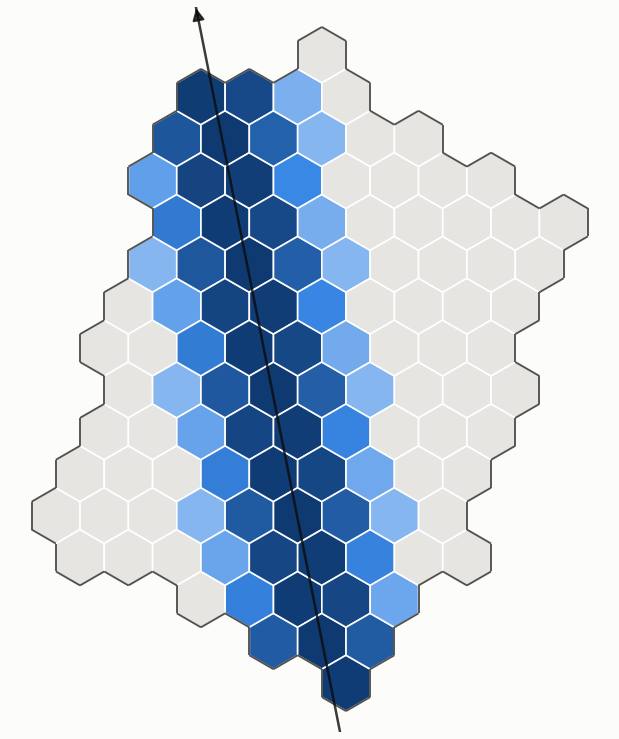
\includegraphics[width=0.62\columnwidth]{concept-river.png}
\caption{The track decides which cell holds which packets. Shade: share of the query that each cell of one cluster
receives from a single pass (darker is more). The ground plan of (P1) moves the missing shares from the dark cells under
the track to the critical cells. \todo{redraw on a forest cluster with critical cells marked.}}\label{fig:recmap}
\end{figure}

\emph{Planning information.} The reception sets $R_c(\omega)$ are known only after the pass, whereas the plan is made
before take-off. (P1) is therefore a two-stage problem. The first stage chooses $(q,s,\bar f)$ on the predicted
reception map $\hat R_c=\{j:P_c(q(t_j))\ge\vartheta\}$ (Fig.~\ref{fig:recmap}); the second stage repairs the plan on the
real reception: gathering and repair within a cell, takeover when the track deviates, and a patch for cells that remain
incomplete.

\emph{Class.} The track part is a Dubins traveling salesman problem with neighbourhoods. For fixed $q$ and reception, the
ground part is a minimum-time multicommodity broadcast schedule on a graph with unit-capacity media, in the family of
minimum broadcast time and minimum-latency broadcast scheduling \cite{you2013}. Relaxing integrality and time gives the
max-load linear programme $\min L$ subject to flow conservation from the cells under the track to the critical cells and
$\sum_{\text{flows through }m}\text{frames}\le L$ for all $m$, whence $\max_kC_k\ge\tau_fL^\star_{\mathrm{LP}}$.

\subsection{(P2) Verification}
Let $A$ be the set of suspected cells, cell $c\in A$ reported at time $r_c$, $p_c(t)$ the posterior and $d(i,j)$ the
flight time of team~2 between cells. The decisions are the take-off time $t_2$ and a policy $\mu$ that, at every
completed verification or new report, picks the next cell from the information available. If all reports were known in
advance, $\mu$ would reduce to a sequence $(c_1,c_2,\dots)$, and with $c^\star=c_{i^\star}$
\begin{equation}
T^\star=t_2+\sum_{i\le i^\star}\bigl(w_i+d(c_{i-1},c_i)+\sigma\bigr),\qquad c_0=\mathrm{BS},\label{eq:tstar}
\end{equation}
where $w_i\ge0$ is the wait if team~2 reaches $c_i$ before $r_{c_i}$. Subject to the endurance of team~2, the problem
is
\begin{equation}
\textbf{(P2)}\quad \min_{t_2,\,\mu}\ Q_{0.9}\bigl[T^\star\bigr]\quad\text{s.t. } t_2\ge\min_{c} r_c,\label{eq:p2}
\end{equation}

\emph{Class.} In the static version with the expected objective, all reports known and $t_2$ fixed, (P2) minimises
$\sum_c p_cL_c$, where $L_c$ is the time at which cell $c$ is verified: the weighted minimum latency (traveling
repairman) problem, the deterministic counterpart of the optimal searcher path problem \cite{trummel1986}. In the
static version with the 0.9-quantile, it asks for the shortest walk from the BS that visits cells of total probability
at least 0.9: a quota TSP whose quota is probability mass, with orienteering as its dual. Release times $r_c$ and
reports that arrive over time make the problem online. Without travel times, visiting cells in decreasing order of $p_c$
is optimal for the expectation (Smith's rule); the greedy policy of our conference version, which ranks cells by $p_c$
divided by travel time, is its travel-aware version.

\subsection{Complexity}
\begin{theorem}\label{thm:nphard}
The decision version of (P1) with deterministic reception, given $T$, is there a plan under which every critical cell
is complete and the UAV is back at the BS by time $T$, is NP-hard. It remains NP-hard for a single UAV of constant
speed and a ground graph without edges.
\end{theorem}
The proof \todo{Appendix A of draft v1} follows Le Ny \emph{et al.}'s reduction for the Dubins TSP \cite{leny2012}:
an instance of Exact Cover is mapped, through Papadimitriou's construction for the Euclidean TSP
\cite{papadimitriou1977} and a rescaling that absorbs both the turning-radius penalty \cite{savla2008} and the
reception radius, to an instance in which every critical cell must be overflown. The theorem locates the hardness in
the flight layer; for fixed $q$ the ground part is hard on its own, and Section~\ref{sec:limits} bounds it from below.

\begin{remark}
(P0) contains the SSCFLP, which is NP-hard \cite{bakker2025}, as the special case described above; the static
expected-value version of (P2) contains the weighted minimum latency problem, which is NP-hard even on weighted trees
\cite{sitters2002}. \todo{state both as propositions with reductions that keep the actual objectives.}
\end{remark}

\section{Limits, Algorithms and Evaluation (to be rewritten)}\label{sec:limits}\label{sec:eval}
\todo{VI Limits; VII Algorithms; VIII Evaluation on forest maps; IX Discussion (mountain parks, multiple UAVs,
density); X Conclusion. Draft v1 holds the urban-agnostic material.}
